\documentclass[11pt]{article}
\usepackage[margin=1in]{geometry}
\usepackage{graphicx}
\usepackage{booktabs}
\usepackage{amsmath}
\usepackage{array}
\usepackage{longtable}
\usepackage{hyperref}
\usepackage{caption}
\usepackage{framed}
\graphicspath{{../figures/}}
\setlength{\parskip}{3pt}
\title{\vspace{-1.8cm}Enrollment evidence for the proposed closure of Mesa Elementary}
\author{Tim Kautz\\ \small PhD economist (Senior Researcher, Mathematica); parent of a Mesa Elementary kindergartner.\\ \small Written in a personal capacity; views are my own. Attachment to a letter to the BVSD Board of Education.}
\date{\small September 2026}
\begin{document}
\maketitle
\vspace{-1.3cm}

\section*{Executive summary}
\begingroup\small\setlength{\parskip}{2pt}
\begin{framed}
\noindent\textbf{The ask.} Decline to approve the Mesa/Bear Creek component of the Resilient Schools proposal on September 22. Ask staff for a one-page Bear Creek worksheet showing how the district's own resident projection becomes the enrollment range in the deck. Every input is public; the calculation is not.
\end{framed}

\noindent\textbf{Five findings}, each from the district's own documents.
\begin{enumerate}
\item \textbf{The step from residents to enrollment is missing, and the district's own data do not supply it.} The proposal projects 522 residents in the combined area in 2030--31 and 403--462 students at Bear Creek (deck p.\ 51). The district's December 2025 Enrollment Pattern Matrix gives the capture rate (the share of the area's resident children attending the two schools), 83\%, and the outside enrollment (students living outside the area, out of district, or placed), 121. At that pattern 522 residents give about 553 students; residents alone give 432, above the floor of the range. Reaching 403--462 needs a capture rate of 54--65\%, which no year since 2017--18 has shown (81--87\%), or removing three-quarters of outside enrollment; under the district's own rules, even with no new outside admissions, the merged school stays above the top of the range in both years (Section~\ref{sec:s1}).
\item \textbf{The district's numbers for these schools move, and the first 2026--27 count is above its projection.} Bear Creek's 2029--30 projection rose 14\% between the January 2025 and January 2026 runs. On August 28, 2026, Bear Creek had 330 students against a projection of 299; the two schools together had 534 against 516 (Section~\ref{sec:s2}).
\item \textbf{The assumption that decides whether the merged school fits is unstated.} An independent model gives 430 or 503 students in 2030--31; the only difference is whether kindergarten intake keeps falling or holds at its recent level. A version built on the district's own births by attendance area gives more, because births there rose from 33 in 2019 to 70 in 2024 (Section~\ref{sec:s4}).
\item \textbf{The fit is a question of classrooms, not seats.} At the district's staffing formula (one teacher per 24.58 students) and at the teachers' agreement's class-size goals, the merged school needs 19--23 classes in 2027--28. The building has 21 classrooms (3.5 rounds) before the RISE and AIM autism programs are housed (Section~\ref{sec:s3}).
\item \textbf{The deck gives no Mesa-specific cost, and the vote is a month earlier than the February and June plans stated.} Those plans set a September study package (boundaries, choice preferences, facility analysis) before an October vote; the deck moves the study to September 8 and the vote to September 22 (Section~\ref{sec:s5}).
\end{enumerate}

\noindent\textbf{What would settle it.} A worksheet listing projected residents by grade, the capture rate assumed, outside enrollment and how policy lets it change, the rooms RISE and AIM occupy, and the classes needed at the staffing formula (Table~\ref{tab:worksheet}). If it shows a fit with margin under the higher cases, the Board has a fair test. Failing a hold, a conditional approval with published triggers on the October 2026 count and the January 2027 run is the weaker form of the same discipline (Section~\ref{sec:s6}).

\noindent\textbf{Conceded.} Mesa is small, has been on the enrollment-advisory list every year it has existed, and the district's projection for it is reasonable. The question is whether the merged school fits the building, and on that the documents presented do not carry the evidence an irreversible decision requires.
\endgroup

\newpage
\section{From residents to enrollment: the missing step}\label{sec:s1}
The proposal's central claim is that Bear Creek ``can house the projected enrollment of both schools in 2027--28 and beyond'' (bvsd.org Resilient Schools page, saved copy p.\ 7). Its figures for the consolidation are on deck p.\ 51: 492 seats; 275 Bear Creek and 228 Mesa residents today (503); 473 residents projected for the combined area in 2027--28 and 522 in 2030--31; and enrollment ranges of 392--445 and 403--462, footnoted as ``dependent on number of resident students from the sending school attending the receiving school.'' The FAQ adds that where new enrollment ``will push the school near capacity,'' projections ``take into account managing choice enrollment beginning in 2027--28'' (p.\ 3). No published document shows the calculation that turns 522 residents into 403--462 students.

The inputs are public. The district's ``Supporting Data'' page lists, as data used to develop the recommendation, its Enrollment Pattern Matrices and School Profile books. The December 5, 2025 elementary matrix gives, for every school, where its students live, and for every attendance area, how many students live there. For the four areas the proposal would combine (Bear Creek, Mesa, and the two optional Bear Creek/Mesa and Bear Creek/Creekside areas) it shows 502 residents, of whom 415 attend Bear Creek or Mesa: a combined-area capture rate of 83\% (own-school 74\%). The other 121 students at the two schools are outside enrollment: 75 in-district choice from outside the area, 23 out-of-district, and 23 placements, whose residence the matrix does not give (treated here as outside, the assumption most favourable to the proposal). The identity $415 + 75 + 23 + 23 = 536$ is the two schools' October 2025 enrollment exactly (Table~\ref{tab:identity}). The 83\% is the latest of nine matrix years and the third-lowest (mean 84\%), so it is a conservative choice; and the deck's 503 residents today equal the four areas' total within one student, so the same geography is assumed for its 522. If the future attendance area is drawn larger than the four areas (deck p.\ 59), some of the 75 in-district choice students would already be among the 522, and the totals below would fall by that number.

\begin{table}[htbp]\centering\footnotesize
\caption{The identity on the district's own matrix (December 5, 2025), and the same pattern applied to the deck's resident projections (p.\ 51).}\label{tab:identity}
\begin{tabular}{p{7.2cm}rrr}
\toprule
 & 2025--26 (matrix) & 2027--28 (473 res.) & 2030--31 (522 res.) \\
\midrule
Residents of the four areas & 502 & 473 & 522 \\
$\times$ combined-area capture (83\%) & 415 & 391 & 432 \\
$+$ in-district choice from outside the area & 75 & 75 & 75 \\
$+$ out-of-district & 23 & 23 & 23 \\
$+$ placements & 23 & 23 & 23 \\
$=$ students at the two schools / merged school & 536 & 512 & 553 \\
\midrule
Proposal's range & & 392--445 & 403--462 \\
Capture needed for the range, outside enrollment held at 121 & & 57--69\% & 54--65\% \\
Outside enrollment needed for the range, capture held at 83\% & & 1--54 & below zero to 30 \\
\bottomrule
\end{tabular}
\end{table}

\begin{figure}[htbp]\centering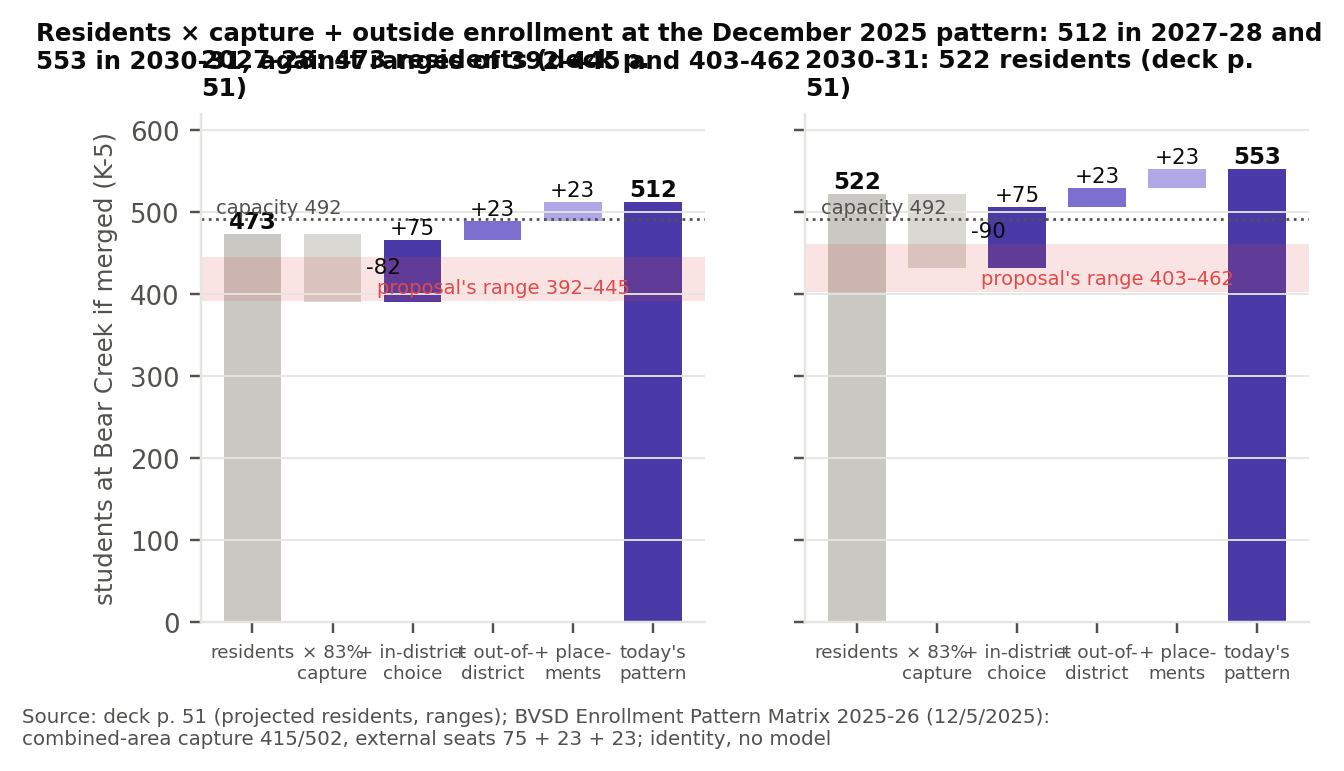
\includegraphics[width=0.92\textwidth]{fig16_bridge.png}
\caption{Residents $\times$ capture $+$ outside enrollment at the December 2025 pattern: 512 in 2027--28 and 553 in 2030--31 against ranges of 392--445 and 403--462. No model is involved. Deck p.\ 51; Enrollment Pattern Matrix 2025--26.}\label{fig:bridge}\end{figure}

Three things follow, none of which depends on any model. First, at today's pattern the merged school is above the building in both years. Second, the range's floor in 2030--31 (403) is below what residents alone would supply at today's capture rate (432): no reduction in outside enrollment reaches it. Third, the top of the range (462) requires either capture of 65\% or outside enrollment cut from 121 to 30. Combined-area capture has been between 81\% and 87\% in every year of the matrix record (Figure~\ref{fig:capture}); 65\% would be a departure from anything observed, and the proposal's own rationale is that a fuller school attracts families, not that it loses a fifth of its residents.

\begin{figure}[htbp]\centering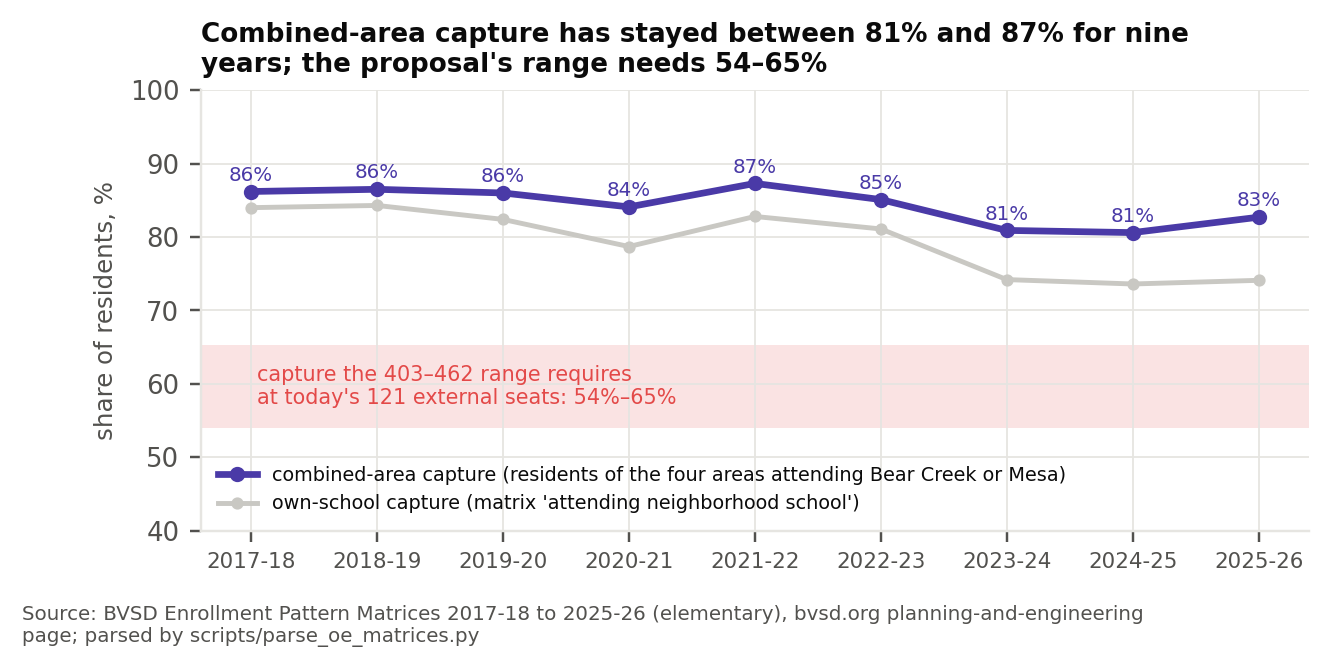
\includegraphics[width=0.9\textwidth]{fig17_capture_history.png}
\caption{Combined-area capture, 2017--18 to 2025--26, and the capture the 403--462 range requires at today's outside enrollment. Enrollment Pattern Matrices (elementary).}\label{fig:capture}\end{figure}

The other lever is outside enrollment, and the district's own rules limit what ``managing choice'' can do. Under policy JECC, open enrollment once granted ``will be approved for the duration of that school level,'' unless assignment ``necessitates adjustments to enrollment at particular schools''; JECC-R sets the lottery preferences. The deck's transition rules (p.\ 63) place in-district students of a closed school in their new neighborhood school, let them apply elsewhere with a one-year priority, and require out-of-district students to apply through open enrollment, with offers that ``depend on available space.'' Applied to the matrix: Bear Creek's own 56 outside students (43 in-district from outside the area, 13 out-of-district) continue and age out one grade a year; the 23 program placements persist, since the programs move to Bear Creek; Mesa's 42 non-resident students have no automatic seat. Under the reading most favourable to the proposal, no new outside admissions and none of Mesa's non-residents re-admitted, the merged school is 461 in 2027--28 and 473 in 2030--31, above the tops of 445 and 462 (Table~\ref{tab:newentrants}); if Mesa's non-residents are re-admitted, 496 and 487; at ten new admissions a year, 471 and 513. The range is reachable only if capture falls as well, or if the district invokes JECC's exception to remove enrolled students, which the record does not show it has done.

\begin{table}[htbp]\centering\footnotesize
\caption{Outside enrollment under the district's transition rules (JECC; deck p.\ 63) with a cap on new outside admissions from 2027--28; residents from deck p.\ 51, capture 83\%. Outside students are assumed spread evenly across six grades; a grade-weighted profile lowers the first row by 4--6 students.}\label{tab:newentrants}
\begin{tabular}{llrrrr}
\toprule
New outside admissions per year & Mesa's 42 non-residents & \multicolumn{2}{c}{2027--28} & \multicolumn{2}{c}{2030--31} \\
 & & outside & merged school & outside & merged school \\
\midrule
None & not re-admitted & 70 & 461 & 42 & 473 \\
None & re-admitted & 105 & 496 & 56 & 487 \\
10 & not re-admitted & 80 & 471 & 82 & 513 \\
About 20 (today's inflow) & not re-admitted & 90 & 481 & 122 & 553 \\
\midrule
Proposal's range & & & 392--445 & & 403--462 \\
\bottomrule
\end{tabular}
\end{table}

The matrix also answers where Mesa's residents go. Of the 176 residents of the Mesa area proper, 118 attend Mesa, 27 attend Bear Creek, 23 attend focus or charter schools, 5 attend other neighborhood schools and 3 are not in the listed school rows. Half of the Mesa-area residents who leave their school go to Bear Creek. The merger reclassifies those 27 as residents attending their own school; it does not recruit them, and it does not touch the 23 at focus schools. The district's own January 2025 boundary work session gave the same picture for the dual Bear Creek/Mesa area: 143 residents, 76 at Bear Creek, 36 at Mesa, 16 at Community Montessori, 15 elsewhere (p.\ 7).

\section{How much the district's numbers move, and the first 2026--27 count}\label{sec:s2}
The district's projections for these two schools have moved 10--14\% between successive annual runs. Bear Creek's 2029--30 projection rose from 272 to 310 (+14\%) between the January 2025 and January 2026 runs while Mesa's fell from 224 to 202 ($-$10\%); Bear Creek's 2028--29 projection went 248, 274, 288 in three runs (Feb.\ 2024 p.\ 11; Feb.\ 2025 p.\ 9; Feb.\ 2026 p.\ 9; Table~\ref{tab:vint} in Appendix~\ref{app:history}). The January 2026 run (printed in the February 2026 report) is the first in which Bear Creek's path turns upward (299, 293, 288, 310, 320), and the documents do not say why; the district's own births table offers a likely reason, taken up in Section~\ref{sec:s4}.

Two measures of accuracy are available. The district scores its own spring projection against each October count; across ten Octobers (2015--2019, 2021--2025) and 328 elementary school-years, the median miss is 3.1\%, one school-year in ten misses by more than 8\%, and the largest miss is 20\% (Appendix~\ref{app:history}). Those are five-to-eight-month horizons. At one and two years, from the three annual runs, one school-level projection in ten misses by more than 9\% and 13\%; four to five years out, four in five revisions between runs are within about 12\% and the largest is 46\%. The district has leaned slightly high on average (+1\%), mostly in 2021 and 2022. The point is not that it projects badly; it is that a five-year point projection for a 220-student school carries a band of several tens of students, and the proposal presents none.

\begin{figure}[htbp]\centering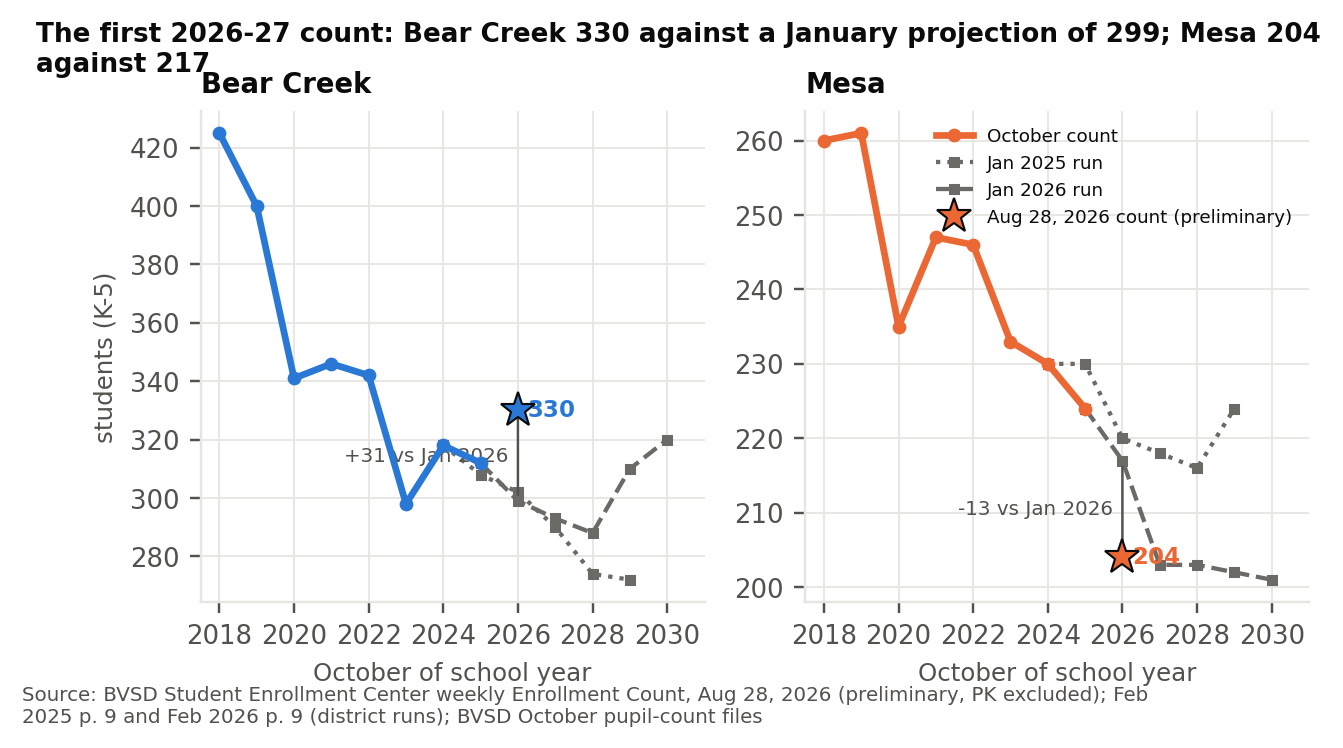
\includegraphics[width=\textwidth]{fig20_aug2026.png}
\caption{The first 2026--27 count: Bear Creek 330 against a January projection of 299; Mesa 204 against 217. Student Enrollment Center weekly count, August 28, 2026 (preliminary); Feb.\ 2026 p.\ 9.}\label{fig:aug}\end{figure}

The first count under the 2026--27 boundaries exists. The Student Enrollment Center's weekly count of August 28, 2026 shows Bear Creek at 330 (+31, +10\% against the January projection of 299) and Mesa at 204 ($-$13, $-$6\% against 217), stable across eight weekly reports since August 4 (Figure~\ref{fig:aug}). The two schools together total 534 against a projected 516 and last October's 536. The count is preliminary: the official count is October 1, August-to-October attrition is unknown, and across the thirty schools the January run covers, August gaps to the projection run from $-$14\% to +10\% with Bear Creek's the largest; the district-wide August total was 0.1\% below the projection and 1.7\% below last October. Bear Creek's first grade (60) is twelve above last year's kindergarten (48), inflow above kindergarten; combined kindergarten is 68, below last year's 76 and the 2023--25 average of 73. Fed into the cohort model as if it were the October count, the August figures raise every merged-school estimate: the 2030--31 central estimate moves from 430 to 450 under the trend assumption and from 503 to 522 under the level assumption, and the share of simulated paths above 492 in the first year moves from 30\% to 48\% and from 52\% to 75\% (Appendix~\ref{app:model}, Table~\ref{tab:cond}). The movement comes from Bear Creek's grades 1--5 sitting about 22 students above what the model expected for 2026, not from the kindergarten refit.

\section{Rooms, not seats}\label{sec:s3}
Bear Creek's 492 seats are ``program capacity based on current use of the building'' (Feb.\ 2026 p.\ 9, footnote). The figure has moved: 475 with 19 possible classrooms in the 2011 School Profile book, 478 with 18 in 2012--2014, 467 (3.0 rounds) in the January 2024 table, and 492 (3.5 rounds, 21 classrooms) from January 2025. Mesa's went from 485 (20 classrooms) and 494 (19) to 418 (3.0 rounds). No document gives the room-by-room basis for any change (Appendix~\ref{app:history}, Table~\ref{tab:capacity}). The bvsd.org page states that ``all existing AIM and RISE programs would be housed at Bear Creek''; the deck that ``Mesa's RISE Program moves to the Bear Creek building'' (p.\ 49). None states how many classrooms these center-based programs occupy at either school or whether 492 nets them out.

Seats are not the operational constraint; classrooms are, and cohorts do not divide evenly into them. Two published figures give the class-size basis. The FY2026--27 budget book prints the elementary staffing formula as one classroom teacher per 24.58 students, a guideline ratio ``with adjustments made to accommodate individual grade levels'' (p.\ 119; PDF p.\ 121); the BVEA agreement prints class-size goals of 26 (K--1), 29 (grades 2--3) and 31 (grades 4--5) (2026--29 agreement \S C-6). The formula is an allocation, not a cap: on the central paths it allocates 19--20 teachers to the merged school in 2027--28. Classes, however, come in whole numbers by grade. For each simulated path of the cohort model (Section~\ref{sec:s4}), the classes needed are the sum over grades of the classes required at each basis (Figure~\ref{fig:sections}, Table~\ref{tab:sections}). At 24.58 students per class, with 90\% of Mesa's students following, the merged school needs 23 classes in 2027--28 under either kindergarten assumption, more than 21 rooms in 73\% (trend) and 85\% (level) of simulated paths; in 2030--31, 21 and 23. At the agreement's ceilings, 19--21 classes, within 21 rooms on the central path. The 21 rooms are themselves derived (3.5 rounds $\times$ 6 grades, the basis of 492); the 2011--14 profile books listed 18--19 ``possible classrooms.'' Neither basis nets out the rooms RISE and AIM occupy. The district can answer with two numbers: which basis the ``three classes per grade'' design uses, and the rooms Bear Creek has after the programs move.

\begin{figure}[htbp]\centering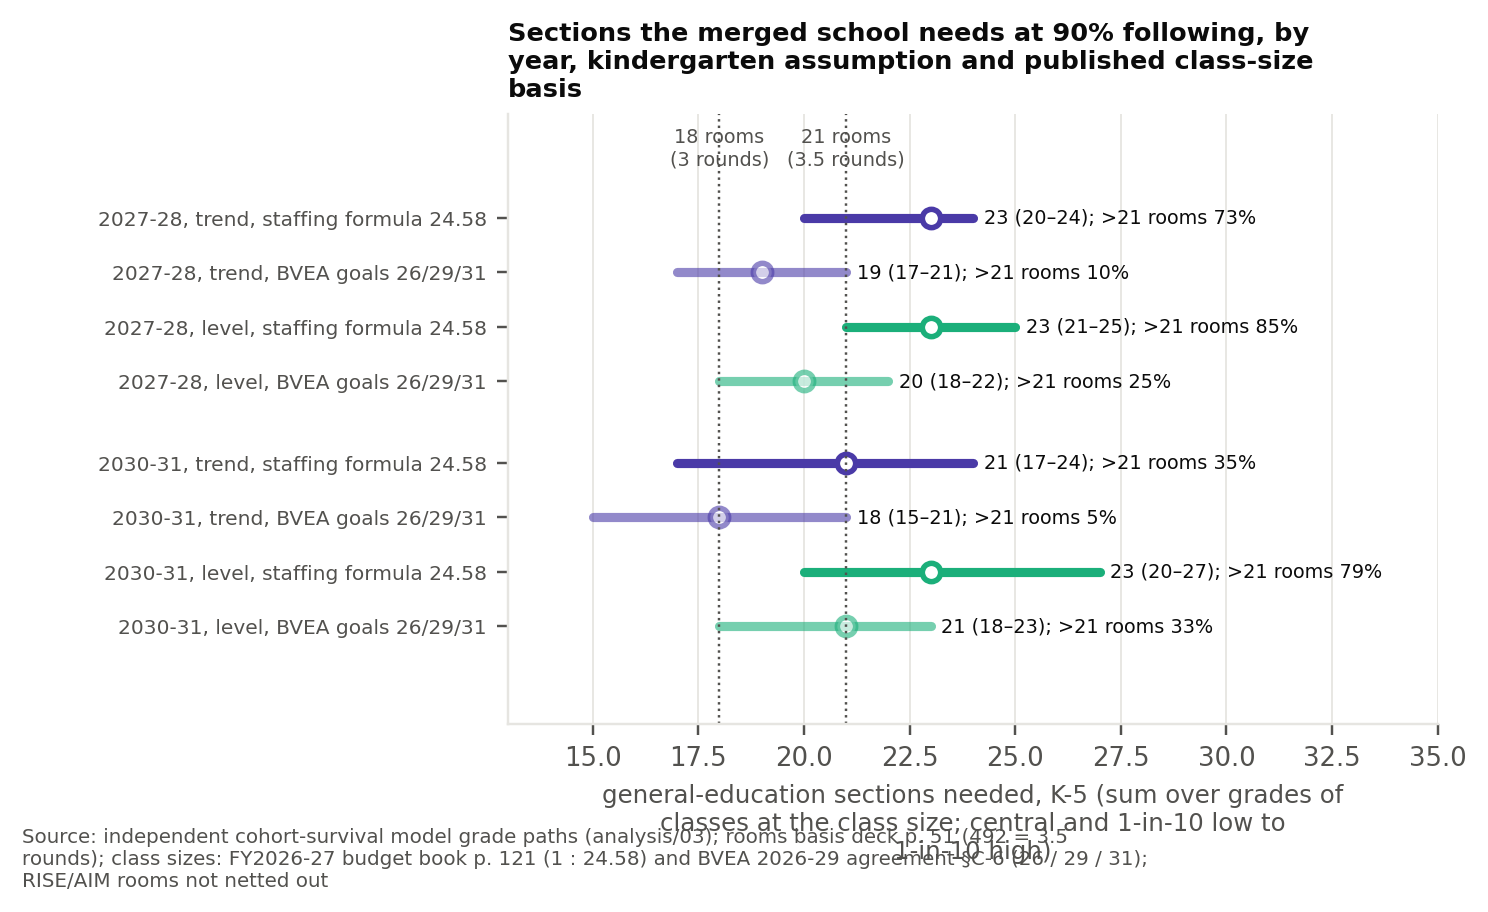
\includegraphics[width=\textwidth]{fig15_sections_by_grade.png}
\caption{General-education sections the merged school needs (sum over grades of classes at the class size), 90\% following, at the staffing formula (solid) and the agreement's goals (faded). Rooms assumed at 21 and 18; RISE and AIM rooms not netted out.}\label{fig:sections}\end{figure}

\begin{table}[htbp]\centering\footnotesize
\caption{Classes needed vs rooms, 90\% following; the last two columns are the share of simulated paths needing more classes than rooms, conditional on the kindergarten assumption and 90\% following.}\label{tab:sections}
\begin{tabular}{lllrrr}
\toprule
Class-size basis & Assumption & Year & Classes, central (low--high) & Over 21 rooms & Over 18 rooms \\
\midrule
Staffing formula 24.58 & Trend & 2027--28 & 23 (20--24) & 73\% & 98\% \\
 & Level & 2027--28 & 23 (21--25) & 85\% & $>$99\% \\
 & Trend & 2030--31 & 21 (17--24) & 35\% & 80\% \\
 & Level & 2030--31 & 23 (20--27) & 79\% & 99\% \\
BVEA goals 26/29/31 & Trend & 2027--28 & 19 (17--21) & 10\% & 70\% \\
 & Level & 2027--28 & 20 (18--22) & 25\% & 85\% \\
 & Trend & 2030--31 & 18 (15--21) & 5\% & 40\% \\
 & Level & 2030--31 & 21 (18--23) & 33\% & 82\% \\
\bottomrule
\end{tabular}
\end{table}

\section{What an independent projection says}\label{sec:s4}
An independent cohort-survival model, patterned on the district's published grade-progression method (Feb.\ 2026 p.\ 7) and fitted to its own grade counts, reports a range. Its one unavoidable choice is kindergarten intake, and that choice decides the answer. Under the \emph{trend} assumption (intake keeps falling on its 2014--25 trend) the merged school with 90\% of Mesa's students following has a 2030--31 central estimate of 430 and a 16\% chance of exceeding 492; under the \emph{level} assumption (intake holds at its 2023--25 average) the central estimate is 503 and the chance is 57\% (Figure~\ref{fig:merged2}). Under either, the chance of a school below two rounds is at most 2\%: the enrollment risk is one-sided, though over-enrollment has remedies (choice limits, boundaries, portables) that under-enrollment lacks, and each of those remedies has a cost the deck does not carry. The district's own Bear Creek projection for 2030--31 (320) sits on the level assumption's central estimate (317), not the trend assumption's (268); its own run puts the two schools together at 521, above the building, so a range of 403--462 is reachable only if 59--118 of those students go elsewhere. Every probability in this document is the share of simulated paths under a stated assumption and a stated share following; they are scenario probabilities, not forecasts.

\begin{figure}[htbp]\centering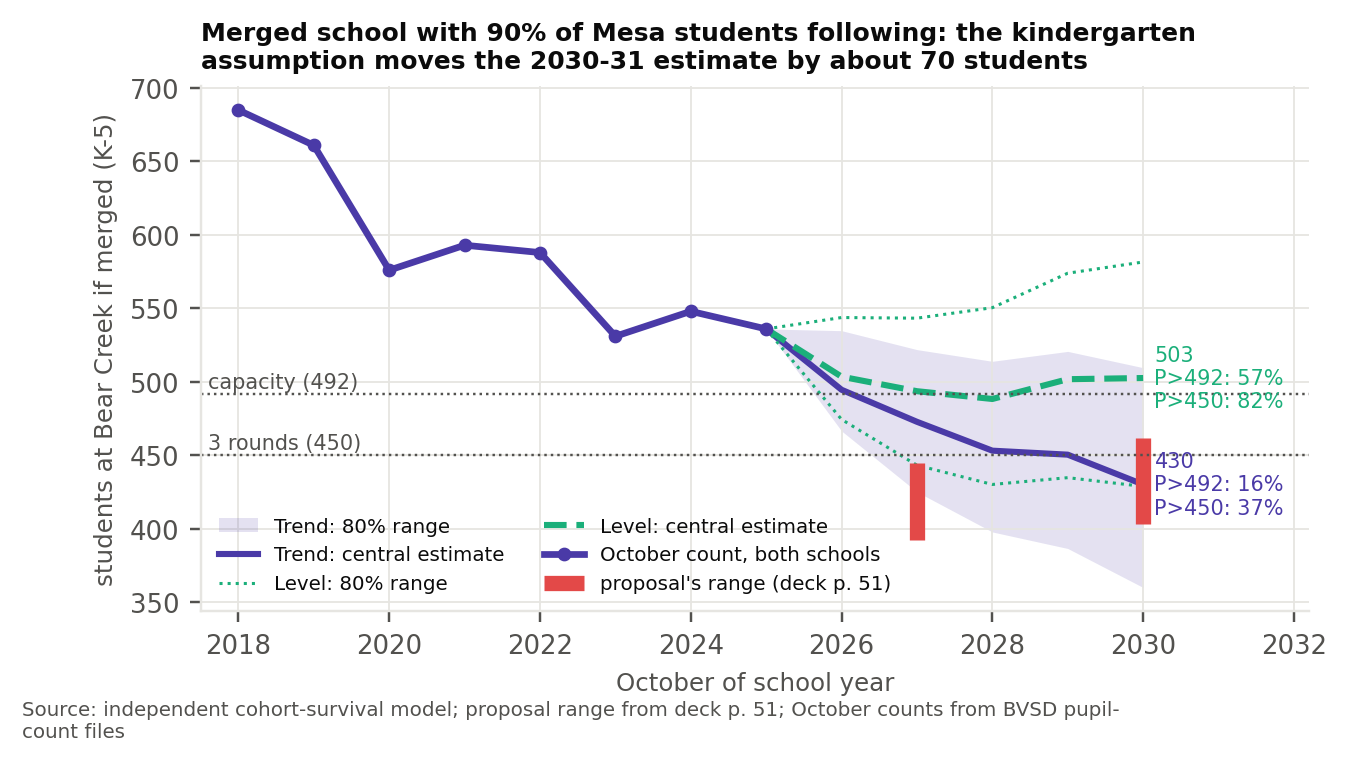
\includegraphics[width=\textwidth]{fig05b_merged_two_specs.png}
\caption{The merged school with 90\% of Mesa's students following, under both kindergarten assumptions, with 80\% ranges, the proposal's range (red) and the 450 and 492 lines.}\label{fig:merged2}\end{figure}

A third specification is possible from the district's own births by elementary attendance area (its annual enrollment packets to the Board). Births in the four South Boulder areas ran 60--88 a year in 2005--14, fell to 33 in 2019, and recovered to 45, 46, 57, 54 and 70 by 2024. Kindergarten at the two schools did not follow the fall: it ran at 1.1 to 1.5 times the areas' births five years earlier through 2023, 2.5 times in 2024 and 1.7 in 2025, because families arrive after birth and choose in (Figure~\ref{fig:births}); the district's method applies its ratio to residents and treats choice separately (Feb.\ 2026 pp.\ 7--8), so the ratios here fold both together. Carrying the district's births forward at the observed entry ratios gives a 2030--31 central estimate of about 505--590 depending on which years' ratios are used: 546 for the full 2014--25 window, 505 if the two most recent, high ratios are excluded, 592 for 2020--25 (Appendix~\ref{app:model}, Table~\ref{tab:births}). The implied 2030 kindergarten (about 90) is above any intake since 2017, so the specification is not offered as a forecast. In every variant the central estimate is at or above the level assumption's 503 students and the top of the district's range: a births-based method does not lower the answer, and it does not make it precise. The district's statement that births ``seem to be leveling'' (news article, Dec.\ 2025) describes Boulder as a whole; in these four areas births have risen since 2019, and the 2024 cohort reaches kindergarten in 2029--30, the year the district's Bear Creek path turns upward.

\begin{figure}[htbp]\centering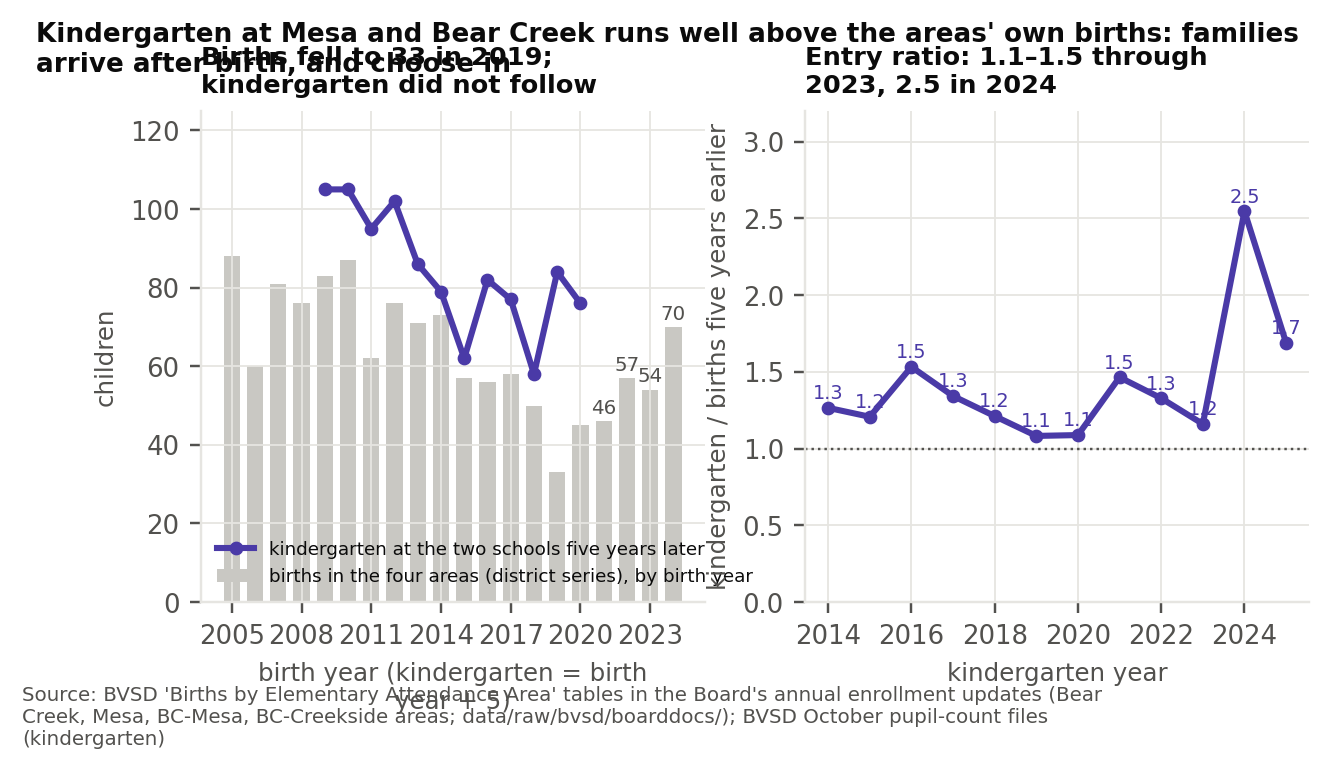
\includegraphics[width=\textwidth]{fig19_births_k.png}
\caption{Births in the four South Boulder areas by birth year and kindergarten at the two schools five years later (left); the entry ratio (right). BVSD births tables in the Board's annual enrollment updates; October pupil-count files.}\label{fig:births}\end{figure}

Three outcomes cannot all happen: a merged school below three rounds, one near three rounds but inside the building, and one above the building. Under either assumption the chance of the middle outcome in 2030--31 is about one in four; the assumptions differ in whether the rest of the probability sits below three rounds (trend) or above the building (level) (Table~\ref{tab:buckets}). The model is not a better forecaster than the district and is not offered as one; back-tested on 26 schools its 80\% ranges caught 72--76\% of outcomes and its errors are the district's size (Appendix~\ref{app:model}).

\section{Cost, process, and what no projection captures}\label{sec:s5}
\textbf{Cost.} The deck gives package-level figures only: recurring savings of \$3.5--4.0M a year against one-time costs of \$7.5--10.0M for facility modifications (``some offset by savings from Bond projects'') and \$5.0M for transition support (p.\ 60). No per-school figure appears on either side. The public record now supplies some. The FY2026--27 budget book gives Mesa a General Fund site budget of \$3.02M for 25.3 staff and 217 projected students, and Bear Creek \$3.69M for 30.5 staff and 299 (per-school pages); the state financial-transparency file gives Mesa's FY2025 general-fund spending as \$3.52M, of which school administration was \$0.36M and building operations and maintenance \$0.29M. Those two lines are the ones that do not follow students; the rest is staffing driven by the formula that moves with them, and the deck does not say what part of the \$3.02M it counts as saved. The package savings are 0.9--1.0\% of General Fund expenditures (\$386.2M in the budget book; \$410.2M on the state summary, which folds in sub-funds) and buy about 23--27 teacher positions at the district's loaded cost, under one per elementary school. Bear Creek and Mesa are both Phase 4 (2026/27) projects of the 2022 bond, with design contracts that went to the Board in November 2025 (Bond oversight update, Feb.\ 2026, p.\ 3); the budget book's bond schedule (printed p.\ 207) lists a Mesa project budget of \$1.38M with \$42,000 spent through 2025 and \$24,000 proposed for 2026--27, completion 2028, and a Bear Creek project of \$2.79M (\$11,000 spent; \$55,000 proposed). The deck does not say what the Mesa project is, whether it proceeds, or whether it is the ``savings from Bond projects'' that offset the facility line. And Bear Creek today ``does not have any general education buses, as the attendance area \ldots\ is within the 1.5 mile walk distance'' (bvsd.org transportation page), while most of the Mesa attendance area lies beyond 1.5 miles of Bear Creek (Appendix~\ref{app:alternatives}); the deck carries no transportation line. Simple payback of the one-time cost from the recurring savings is 3.1 to 4.3 years if the savings are realized in full. Read against the standalone projections, the range corresponds to 29--59\% of Mesa's projected enrollment not appearing at Bear Creek, and the deck does not say where those students go or what funding follows them.

\textbf{Process.} The February 2026 trend report set ``Present final plan for study to the Board'' for September 2026 and ``Present final plan for action'' for October (p.\ 13); the June 9, 2026 Board update listed the same two steps, with the study package to ``include updated attendance boundaries, open enrollment preferences, analysis of facility improvements required (if any)'' (p.\ 37), and the district's first community message said final action was ``planned for October.'' The deck's own timeline moves both steps a month earlier, study on September 8 and action on September 22, ``necessary for BVSD open enrollment timeline beginning Nov.\ 1'' (p.\ 70); no document gives another reason. The August 25 agenda item carries one attachment, the 75-page deck; the study package, if it comes on September 8, arrives fourteen days before the vote. On the open-enrollment priority every range depends on, the FAQ says ``The Board will study this item further on Sept.\ 8'' (p.\ 2). The district has itself held one component of the proposal ``for further study'' (dual-language schools, deck p.\ 72).

\textbf{Interdependence.} Every projection here, the district's and this one, is fitted on flows observed under the current portfolio and choice rules. The proposal closes Douglass, Flatirons and Birch, relocates two focus schools and redraws attendance areas across the region (deck pp.\ 23, 46, 52, 59), and gives students of closed schools a one-year open-enrollment priority (p.\ 63). After the package, the Boulder-region neighborhood schools projected at or near three rounds are Foothill (484--492) and Bear Creek at the top of its range; among the ten receiving schools in the proposal, Bear Creek's 2030--31 range is the widest (59 students; next 37) and its margin at the top the smallest (30 seats; Superior's is 31, and Superior's 2027--28 margin is smaller still) (Appendix~\ref{app:claims}, Table~\ref{tab:widths}). The channels run both ways; the documents do not say which historical flows are assumed to persist, and none is modeled here.

\section{What the Board should ask for}\label{sec:s6}
The request is not for a new forecasting system. It is for the assumptions already behind the recommendation to be put into one auditable reconciliation. Table~\ref{tab:worksheet} lists the rows; most draw on data the district already publishes.

\begin{table}[htbp]\centering\small
\caption{The Bear Creek worksheet: rows the Board can ask staff to supply before the vote.}\label{tab:worksheet}
\begin{tabular}{p{2.5cm}p{5.5cm}p{6.0cm}}
\toprule
Block & Field & What it resolves \\
\midrule
Definitions & Projection vintage; exact geography of the future attendance area; definition of ``resident'' & Whether the 522 residents are the matrix's four areas (502 today) \\
Resident demand & Residents by grade, K--5: low, central, high, and the births and entry ratios behind them & The 503 $\to$ 473 $\to$ 522 path against the observed 733 $\to$ 502 \\
Resident capture & Combined-area capture assumed, by year & The 83\% today against the 54--65\% the range requires \\
Outside enrollment & In-district choice from outside the area, out-of-district and placements assumed, by year; new admissions per year; how JECC's continuing-enrollment rule and the deck's p.\ 63 transition rules are applied & The 121 today against the 30 the top of the range requires \\
Reconciliation & Residents $\times$ capture $+$ outside enrollment $=$ 403 and 462 & The bridge \\
Program space & Rooms for RISE, AIM, specials, intervention, preschool, school-age care & Whether 492 is operationally meaningful \\
Sections & Sections needed by grade at the staffing formula, low, central, high; usable rooms after the programs move & Fit and margin \\
Uncertainty & The district's own error record at one to five years; the October 2026 count & Whether the margin is large relative to forecast error \\
Contingency & The count or room result that would trigger more sections, choice limits or reconsideration & A response if the high case occurs \\
Fiscal & Mesa-specific recurring savings, one-time costs, transportation, the Mesa bond project & Net benefit of this component \\
\bottomrule
\end{tabular}
\end{table}

\noindent\textbf{A second-best course.} If the Board is unwilling to hold the component, the alternative that respects the uncertainty is approval with published triggers. The October 2026 count is weeks away and the January 2027 run follows. The Board could adopt the component subject to reconsideration if the October count for the two schools exceeds a stated figure or if the January 2027 run's merged-school range, net of program rooms, tops 462 or centers above 450; the preliminary August count already exceeds the January 2026 figure for the two schools. The values are for the Board to set and staff to state; what matters is that they are written down before the vote. The cost of meeting the standard is one enrollment cycle: the September 22 action is tied to the November 1 choice window (deck p.\ 67), so a decision after the October count takes effect in 2028--29 at the earliest.

\appendix
\section{The evidence standard}\label{app:standard}
An irreversible decision should be held to a higher bar than a reversible one. Closing a school cannot be undone; keeping one open can. Before approving any closure the Board should have in hand: (i) a projection for the merged school with a stated interval, back-tested against the district's own October counts; (ii) the capture, outside-enrollment and continuing-enrollment (JECC) assumptions behind any merged-school range, stated explicitly; (iii) a demonstration that the merged school fits the receiving building with margin under the upside cases, shown in sections at the published staffing formula and net of program rooms; (iv) a school-specific accounting of one-time costs, recurring savings, transportation and revenue at risk; (v) a transition plan for RISE, school-age care, preschool and transportation. The standard applies to every component of the package; this document covers the one its author can speak to. Terms: \emph{run}, the district's annual January projection; \emph{October count}, the state count, K--5; \emph{round}, one class per grade, about 150 students; \emph{combined-area capture}, the share of the four areas' residents attending Bear Creek or Mesa; \emph{outside enrollment}, students enrolled from outside the four areas, out-of-district, and placements; \emph{trend} and \emph{level} assumptions, kindergarten intake on its 2014--25 trend or at its 2023--25 average; \emph{central estimate}, the median of simulated outcomes; \emph{80\% range}, the 1-in-10 low to the 1-in-10 high.

\section{The district's plan, claim by claim}\label{app:claims}
Each row sets a claim in the proposal against the public record. Nothing here asserts a reason; each ends with the question staff can answer.

\begin{small}
\begin{longtable}{p{3.6cm}p{6.6cm}p{4.2cm}}
\toprule
Claim (where) & What the record shows & Question for staff \\
\midrule
\endhead
Bear Creek ``can house the projected enrollment of both schools'' (bvsd.org p.\ 7; deck p.\ 51) & On the matrix and the deck's residents, today's pattern gives 512 and 553; the range needs capture no year has shown or a cut of three-quarters of outside enrollment (\S\ref{sec:s1}). & The worksheet (Table~\ref{tab:worksheet}). \\
Combining the areas ``provides the resident student population for a three-round school'' (bvsd.org p.\ 7) & $522 \times 83\% = 432 < 450$; the three-round school depends on the outside enrollment the FAQ says will be managed. & What outside enrollment the design assumes. \\
Residents 503 $\to$ 473 $\to$ 522 (p.\ 51); chart $\approx$445 in 2030 (p.\ 44) & The four areas' residents fell 733 $\to$ 502 since 2017--18 (matrix totals); the deck's 503 equals the matrix's four-area total, so the definitions reconcile, but the projected rise does not come from any document. & The basis of 522: births, housing, or migration. \\
``Mesa is projected to continue to decline''; second-lowest resident count (p.\ 50) & Conceded on enrollment. Bear Creek's own area lost residents faster (254 $\to$ 162, $-$36\%) than Mesa's (227 $\to$ 176, $-$22\%). & None; context. \\
63\% utilization (p.\ 50); 492 seats, 3.5 rounds (p.\ 51; Feb.\ 2026 p.\ 9) & 475--478 with 18--19 classrooms in 2011--14; 467 in Jan.\ 2024; 492 (21 rooms, derived) since Jan.\ 2025; Mesa 485--494 $\to$ 418 (Table~\ref{tab:capacity}). & The room-by-room basis; the AIM/RISE footprint. \\
Range ``dependent on \ldots\ resident students \ldots\ attending'' (p.\ 51) vs ``take into account managing choice enrollment'' (FAQ p.\ 3) & Two descriptions of the same range; JECC continues existing open enrollment for the school level, so management acts on new entrants (Table~\ref{tab:newentrants}). & Which, and at what level, for Bear Creek. \\
``Reduces excess capacity''; ``10 schools needed'' (p.\ 43); 14 $\to$ 6 (p.\ 58); 67.9\% (p.\ 55) & Mesa is 418 of 1,906 seats; 13 Boulder schools remain; the 6 and the 67.9\% do not reproduce from the deck's own ranges (App.~\ref{app:history}). & Definitions; whether a further round is intended. \\
\$3.5--4.0M recurring; \$7.5--10.0M $+$ \$5.0M one-time (p.\ 60) & No Mesa figure in the deck; Mesa's FY27 site budget is \$3.02M, of which the non-following lines (administration, building operations) were about \$0.65M in FY2025; the package saving is 0.9--1.0\% of General Fund spending; Bear Creek and Mesa are 2026/27 bond projects; no transportation line; press reports about half the facility figure budgeted for next year (Boulder Reporting Lab, Aug.\ 25). & By-school lines; the bond offset; the Mesa project; transportation; the vacant building's carrying cost. \\
``Managing choice'' as the remedy for the upside case (FAQ p.\ 3) & JECC continues granted open enrollment for the school level (with an exception for enrollment adjustments the record does not show invoked); deck p.\ 63 gives Mesa's non-residents no automatic seat; even so the merged school stays above the range tops with no new admissions. & The new-admission level assumed for 2027--28 to 2030--31. \\
Study in September, action in October (Feb.\ 2026 p.\ 13; June 9, 2026 update p.\ 37; district message) vs study Sept.\ 8, action Sept.\ 22 (deck pp.\ 3, 70) & The deck moves both steps a month earlier, citing the Nov.\ 1 open-enrollment window; the study package listed in February and June arrives at most fourteen days before the vote. & The reason for the change; the study package. \\
Open-enrollment priority: ``The Board will study this item further on Sept.\ 8'' (FAQ p.\ 2) & Every range assumes it. & Settle it before any dependent component. \\
Program space: RISE/AIM rooms; preschool ``by Oct.\ 1'' (deck p.\ 64); school-age care (FAQ p.\ 5) & Not stated in any document. & Rooms and locations before the vote. \\
K-2 / 3-5 option ``studied'' (p.\ 56); fiscal impact ``uncertain'' (Oct.\ 2025 slide 45) & No comparison published (Table~\ref{tab:k25}). & The comparison. \\
Projection method: cohort survival with births (Feb.\ 2026 p.\ 7); no interval & Own scoring: median miss 3\%, one in ten above 8\%, at five to eight months; one in ten above 13\% at two years; Bear Creek already 10\% above the January figure in August 2026. & Kindergarten and birth inputs for these two schools; the Jan.\ 2026 upturn. \\
\bottomrule
\end{longtable}
\end{small}

\noindent\textbf{Package-wide items that bear on Bear Creek's fit.} Each post-change range carries the same footnote (pp.\ 25, 37, 48, 51, 54). Decoded against the Feb.\ 2026 standalone projections, the ranges imply that 82--100\% of Birch's students land at Kohl, 82--96\% of Flatirons' at Foothill and Whittier, 84--100\% of Douglass's at its three receivers, but 55--71\% of Monarch K--5's and 41--71\% of Mesa's (2030--31; Figure~\ref{fig:shares}). The two components with the lowest implied shares are the two whose receiving buildings would otherwise be at or over capacity, consistent with the FAQ's statement that choice enrollment would be managed where schools near capacity; which reading applies is not stated. Program capacity was restated for seven schools across the three annual tables, in both directions (Bear Creek 467 $\to$ 492, Coal Creek 516 $\to$ 492, Douglass 442 $\to$ 418; Kohl 516 $\to$ 541, Aspen Creek 461 $\to$ 442, Community Montessori 392 $\to$ 369, Louisville 615 $\to$ 590); the tables give no basis, and the utilization thresholds on which advisory status turns are computed on these denominators. Monarch 6--8's capacity is undetermined (p.\ 39). Every post-change utilization percentage on pp.\ 25, 37, 39, 48, 51 and 54 reproduces from its own range and capacity; the Feb.\ 2026 table's totals and advisory counts reproduce; the capacity reduction of 1,906 reproduces; Mesa's and Bear Creek's counts reconcile exactly across twelve years of files.

\begin{table}[htbp]\centering\small
\caption{Post-change enrollment ranges printed in the deck for 2030--31, ten receiving schools, sorted by width (deck pp.\ 25, 37, 48, 51, 54; capacities Feb.\ 2026 p.\ 9).}\label{tab:widths}
\begin{tabular}{lrrrr}
\toprule
School & Capacity & Range 2030--31 & Width & Seats left at top \\
\midrule
Bear Creek (receives Mesa) & 492 & 403--462 & 59 & 30 \\
Kohl (receives Birch) & 541 & 437--474 & 37 & 67 \\
Coal Creek & 492 & 395--427 & 32 & 65 \\
Eldorado K--5 & 568 & 353--377 & 24 & 191 \\
Whittier & 442 & 315--329 & 14 & 113 \\
Superior & 467 & 424--436 & 12 & 31 \\
Fireside & 516 & 421--430 & 9 & 86 \\
Foothill & 565 & 484--492 & 8 & 73 \\
Heatherwood & 492 & 260--268 & 8 & 224 \\
Eisenhower & 492 & 297--302 & 5 & 190 \\
\bottomrule
\end{tabular}
\end{table}

\begin{figure}[htbp]\centering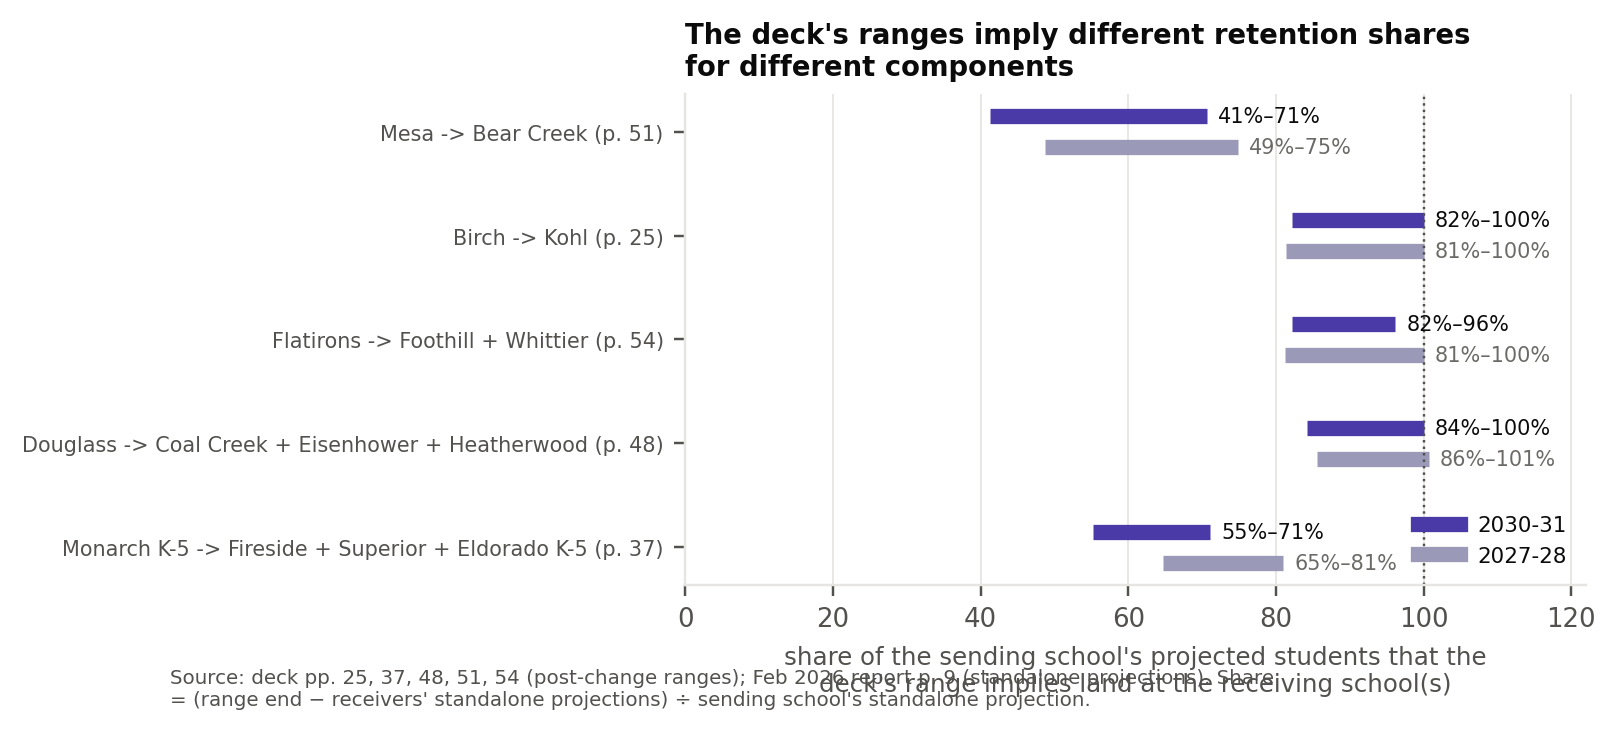
\includegraphics[width=\textwidth]{fig13_package_implied_shares.png}
\caption{Share of each sending school's projected students that the deck's post-change range implies land at the receiving school(s), decoded against the Feb.\ 2026 standalone projections.}\label{fig:shares}\end{figure}

\section{Data, sources and verification}\label{app:data}
Every number traces to a page of a BVSD, Colorado Department of Education, State Demography Office or Census document held unmodified under \texttt{data/raw/}: the Aug.\ 25, 2026 deck; the February 2024, 2025 and 2026 trend reports; the Oct.\ 21, 2025 work session; the boundary items of Jan.\ 14, Mar.\ 11, May 20 and Sept.\ 9, 2025; BVSD's October pupil-count files 2014--15 to 2025--26; CDE membership files 2019--20 to 2025--26; the Enrollment Pattern Matrices 2016--17 to 2025--26 and School Profile books 2011--2025 from the district's planning page; the Student Enrollment Center's weekly 2026--27 counts; the Board's annual enrollment packets 2015--2025 with their projection-vs-count and births-by-area tables; the FY2025--26 and FY2026--27 budget books; Board policies JC, JECC and JECC-R; the BVEA 2026--29 agreement; the 2022 bond oversight update; the bvsd.org Resilient Schools, FAQ, supporting-data and transportation pages; and the district's Dec.\ 2025 enrollment news article. The capacity tables in the trend reports are images and were OCR'd and checked by eye; the 2025--26 matrix rows for both schools were checked cell by cell against the rendered page; the matrix identities hold in every parsed year; grade counts sum to head counts in all twelve years; CDE and BVSD agree within one or two students. Where sources disagree (three definitions of ``resident'', the p.\ 44 chart, School Profile editions, press figures, birth-period definitions) both are recorded in \texttt{data/CONFLICTS.md}. Detail: \texttt{data/SOURCES.md}, \texttt{data/VERIFICATION.md}.

\section{Enrollment history, projection record and capacity}\label{app:history}
\begin{table}[htbp]\centering\small
\caption{BVSD projections by run and target year (K--5). Feb.\ 2024 p.\ 11; Feb.\ 2025 p.\ 9 (re-printed as Oct.\ 2025 work session slide 17); Feb.\ 2026 p.\ 9; October counts from the pupil-count files; Aug.\ 28, 2026 from the weekly count (preliminary).}\label{tab:vint}
\begin{tabular}{llrrrr}
\toprule
School & Target year & Jan 2024 run & Jan 2025 run & Jan 2026 run & Count \\
\midrule
Bear Creek & 2024--25 & 287 & 318 & -- & 318 \\
 & 2025--26 & 273 & 308 & 312 & 312 \\
 & 2026--27 & 271 & 302 & 299 & 330 (Aug.) \\
 & 2027--28 & 262 & 290 & 293 & \\
 & 2028--29 & 248 & 274 & 288 & \\
 & 2029--30 & -- & 272 & 310 & \\
 & 2030--31 & -- & -- & 320 & \\
\midrule
Mesa & 2024--25 & 220 & 230 & -- & 230 \\
 & 2025--26 & 211 & 230 & 224 & 224 \\
 & 2026--27 & 202 & 220 & 217 & 204 (Aug.) \\
 & 2027--28 & 203 & 218 & 203 & \\
 & 2028--29 & 202 & 216 & 203 & \\
 & 2029--30 & -- & 224 & 202 & \\
 & 2030--31 & -- & -- & 201 & \\
\bottomrule
\end{tabular}
\end{table}

\paragraph{The district's own scoring.} Each December the district sets its spring planning projection against the October count for every school (plotted in \texttt{figures/fig21}). Across 328 elementary school-years in ten Octobers (2015--2019, 2021--2025; Gold Hill, Jamestown and online programs excluded), the median absolute miss is 3.1\%, the 80th percentile 6.5\%, the 90th 8.2\% and the largest 20\%; the average signed miss is +1.1\%, so the district has leaned slightly high, mostly in 2021 and 2022, whose misses also supply most of the tail (without those two years the 90th percentile is 7.7\%). School-years within a year share shocks, so these are pooled shares of school-years, not per-school probabilities. Schools under 300 students miss more (median 3.8\%, 90th percentile 8.8\%) than schools over 400 (2.5\%, 7.5\%). Bear Creek's ten misses have a median of 2.9\% and a maximum of 8.0\% (2018: 459 projected, 425 counted); Mesa's a median of 3.6\% and a maximum of 7.3\% (2022). The horizon is short: the projections are dated February to May of the same year, and January 23 for 2025, so the 2025 case is the January 2025 run also scored in Table~\ref{tab:err}.


\paragraph{One and two years ahead, and revisions.} From the three annual runs, 59 one-year and 29 two-year cases can be scored (Table~\ref{tab:err}; the distributions are plotted in \texttt{figures/fig03} and \texttt{fig04}). District-wide totals are projected well ($-$1.1\%, $-$0.7\%, +1.4\%); the school-level errors are what school-level projections look like when resident moves, open enrollment and small numbers all contribute. The 29 two-year cases all score one run against one October, so they are not independent tests, and revisions as a guide to longer horizons assume later revisions are not reversed; on that assumption they are a lower bound.

\begin{table}[htbp]\centering\small
\caption{Absolute percent error of BVSD school-level projections from the annual runs, and magnitude of revisions to the same target year between successive runs.}\label{tab:err}
\begin{tabular}{lrrrrrr}
\toprule
 & $n$ & Median & 80th pct. & 90th pct. & Max & Average error (sign kept) \\
\midrule
Error, 1 year ahead & 59 & 3.2\% & 6.4\% & 9.4\% & 20.2\% & +0.6\% \\
Error, 2 years ahead & 29 & 5.7\% & 9.4\% & 13.0\% & 17.6\% & 0.0\% \\
Revision, target 2 years out & 59 & 3.9\% & 9.1\% & 11.5\% & 24.9\% & \\
Revision, target 3 years out & 59 & 6.0\% & 10.8\% & 12.3\% & 27.4\% & \\
Revision, target 4 years out & 59 & 6.2\% & 12.2\% & 15.1\% & 32.8\% & \\
Revision, target 5 years out & 59 & 6.5\% & 12.5\% & 14.7\% & 46.1\% & \\
\bottomrule
\end{tabular}
\end{table}



\paragraph{Residents.} The matrix's column totals give the residents of each attendance area. For the four areas that would form the combined area they run 733, 706, 688, 592, 592, 583, 535, 526, 502 from 2017--18 to 2025--26 ($-$32\%); kindergarten-age residents 104 to 70 (Figure~\ref{fig:residents}). The deck's 503 for today equals the four-area total within one student; its 473 for 2027--28 and 522 for 2030--31 reverse the direction of eight years of the district's own counts. Boulder-wide, the deck projects residents falling 9\% by 2030 (p.\ 43). The Bear Creek area proper fell from 254 to 162 residents and the Mesa area from 227 to 176. Three definitions of ``resident'' circulate (the matrix's area-proper counts, the School Profile books' ``neighborhood students'' of 264 and 220, and the deck's 275 and 228); every capture rate in this document names its denominator.

\begin{figure}[htbp]\centering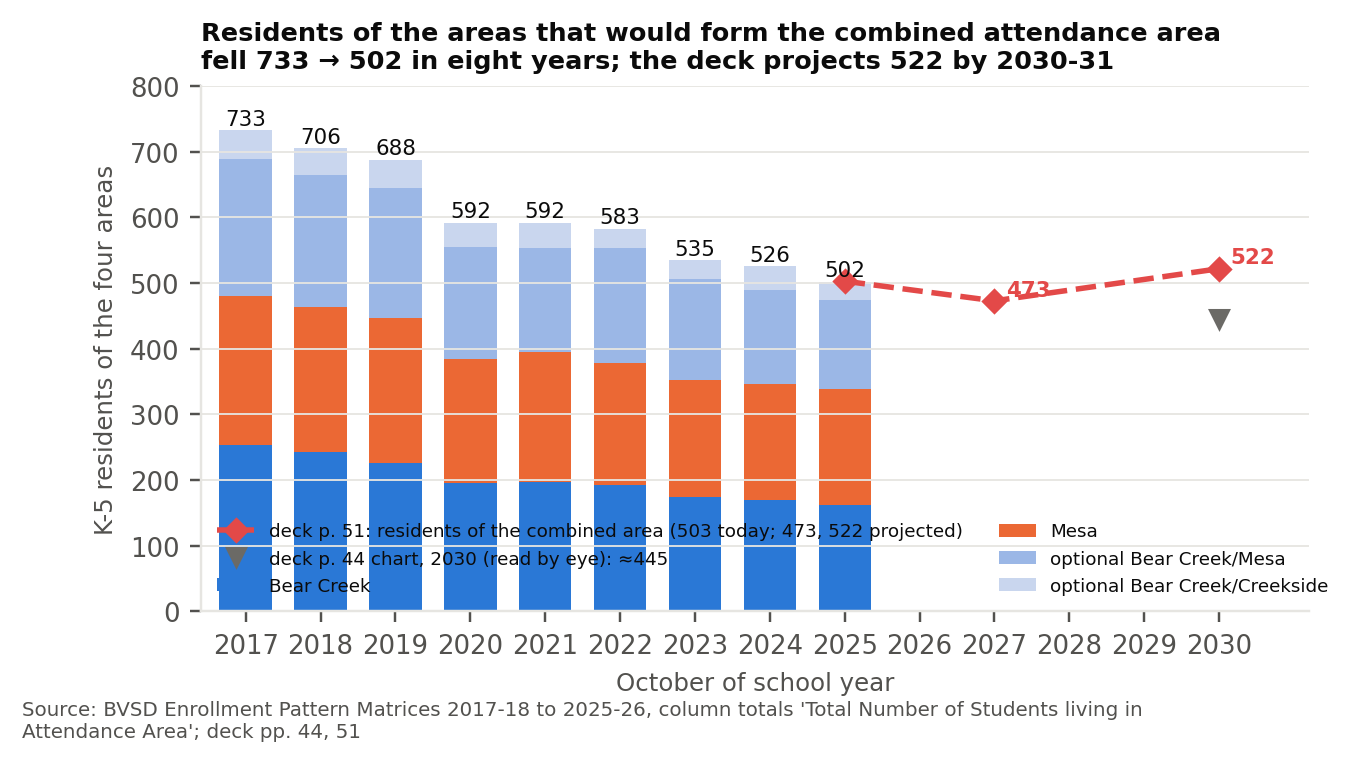
\includegraphics[width=\textwidth]{fig18_residents.png}
\caption{Residents of the four areas, 2017--18 to 2025--26, against the deck's 503, 473 and 522 (p.\ 51) and the p.\ 44 chart's 2030 value.}\label{fig:residents}\end{figure}

\begin{table}[htbp]\centering\footnotesize
\caption{Program capacity of the two buildings as stated by the district over time. School Profile books (2011, 2012, 2014); trend-report capacity tables (Feb.\ 2024 p.\ 11; Feb.\ 2025 p.\ 9; Feb.\ 2026 p.\ 9).}\label{tab:capacity}
\begin{tabular}{llrrr}
\toprule
School & As of & Capacity & Classrooms & Rounds \\
\midrule
Bear Creek & 2011 (Profile book 2011) & 475 & 19 & \\
 & 2012 (Profile books 2012, 2014) & 478 & 18 & \\
 & Jan.\ 2024 (Feb.\ 2024 report) & 467 & & 3.0 \\
 & Jan.\ 2025, Jan.\ 2026 (Feb.\ 2025, 2026 reports) & 492 & 21 (3.5 $\times$ 6) & 3.5 \\
Mesa & 2011 (Profile book 2011) & 485 & 20 & \\
 & 2012 (Profile books 2012, 2014) & 494 & 19 & \\
 & Jan.\ 2024 to 2026 & 418 & & 3.0 \\
\bottomrule
\end{tabular}
\end{table}

\paragraph{Other figures that do not reproduce.} ``14 to 6 schools below two classes per grade'' (p.\ 58): the 14 reproduces from the Feb.\ 2026 table; after the package the schools projected below 300 in 2030--31 are Heatherwood, Creekside, Community Montessori and Sanchez plus the three mountain schools, with Eisenhower at the low end of its range, so four to seven depending on definitions the deck does not give. ``67.9\%'' post-change Boulder utilization (p.\ 55): removing the capacity the package closes and using the deck's own 2030 enrollment gives 71.9\%. Deck ``current'' enrollments differ from the October count by one or two for Birch, Fireside and Aspen Creek.

\section{The independent model}\label{app:model}
\paragraph{Method.} Grade-progression rates $g_{i,t} = N_{i,t}/N_{i-1,t-1}$ for grades 1--5 and years 2015--2025 for each school. Trend assumption: $\log K_t = a + b\,t + e_t$ fitted on 2014--2025, with $(a,b)$ resampled by a pairs bootstrap for each simulated path and $e$ drawn from the fitted residuals. Level assumption: $\log K_t = \log \bar K + e_t$, $\bar K$ the mean of a bootstrap resample of the 2023--25 intakes and $e$ the residual series centered on its mean. In each simulated year one historical year is drawn and its residual and all five rates are applied to both schools, so a shock like 2020 stays one event. Ten thousand paths to fall 2030. Merged enrollment is Bear Creek's path plus a share $r$ of Mesa's, drawn jointly. Births assumption (new): $K_{s,t} = B_{t-5} \times \rho_{s,w}$, with $B$ the district's births in the four areas and $\rho$ the school's observed entry ratio in a window year $w$ drawn each year (windows 2014--25 and 2020--25); $B_{2025}$ is not yet published and is set at $B_{2024}$ scaled by the county's 2025/2024 change. The check model is a random walk with drift on log total enrollment.

\paragraph{Backtest.} Fitted through October 2023 and October 2024 and scored on the counts that followed, for the 26 elementary schools with complete 2014--2025 records. Coverage of the nominal 50 / 80 / 95\% ranges: trend 40 / 74 / 88\% one year ahead ($n=50$) and 32 / 72 / 88\% two years ahead ($n=25$); level 48 / 76 / 92\% and 32 / 72 / 88\%. Median absolute error of the central estimate, one and two years: trend 3.3\% and 8.4\%, level 4.0\% and 6.5\%, against the district's 3.3\% and 5.7\% on the same school-years. Average signed error at two years: trend $-$0.6\%, level +3.0\%; the two err in opposite directions, which is the reason to show both. For Bear Creek, the trend assumption fitted through 2023 gave 282 and 265 against actuals of 318 and 312, outside its 80\% range both years; the level assumption gave 292 and 288, inside. The 80\% coverage is not distinguishable from 80\% at these sample sizes, with a thin upper tail at two years, and the cases are not independent, so the backtest fails to refute calibration rather than establishing it (Figure~\ref{fig:bt}).

\begin{figure}[htbp]\centering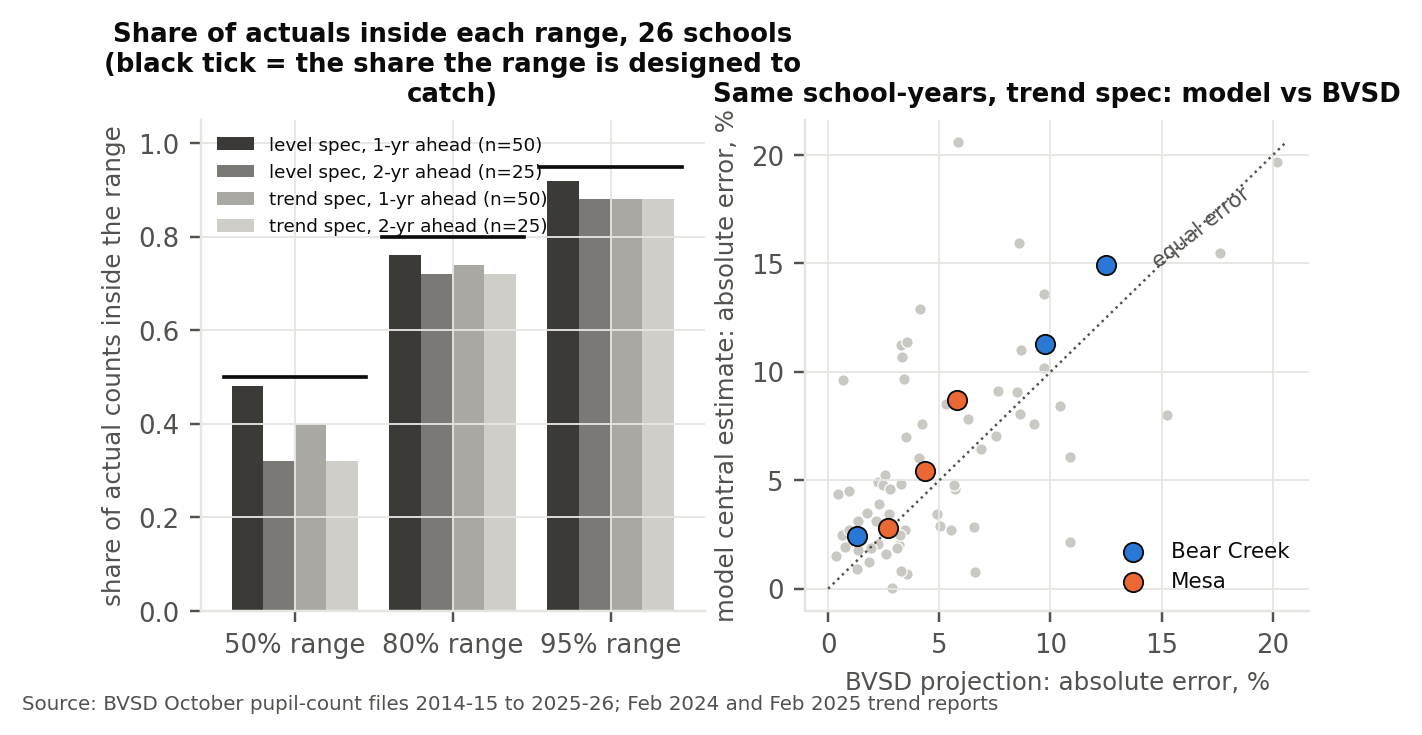
\includegraphics[width=\textwidth]{fig06_backtest.png}
\caption{Backtest across 26 schools: share of actual counts inside each range under both assumptions (left; black tick = designed coverage), and the model's errors against the district's on the same school-years (right).}\label{fig:bt}\end{figure}

\paragraph{Why the kindergarten assumption is the fork.} Combined intake at the two schools was 105, 105, 95, 102, 86 and 79 in 2014--2019, stepped down to 62 in 2020, and has been 82, 77, 58, 84, 76 since, with 68 on the August 2026 count. A trend fitted through a step-then-plateau extrapolates a decline that on this evidence ended five years ago: under the trend assumption Bear Creek's first simulated kindergarten class (central 39) sits below four of the last five observed intakes. At the observed grade-to-grade gains about 69 a year fills 492 seats in steady state; the 2023--25 average is 73 (Figure~\ref{fig:kinder}). The level estimate is sensitive to its window: 505--547 for two- to six-year windows, 484 with median-centered noise; under every variant the central estimate is at or above the top of the district's range.

\begin{figure}[h]\centering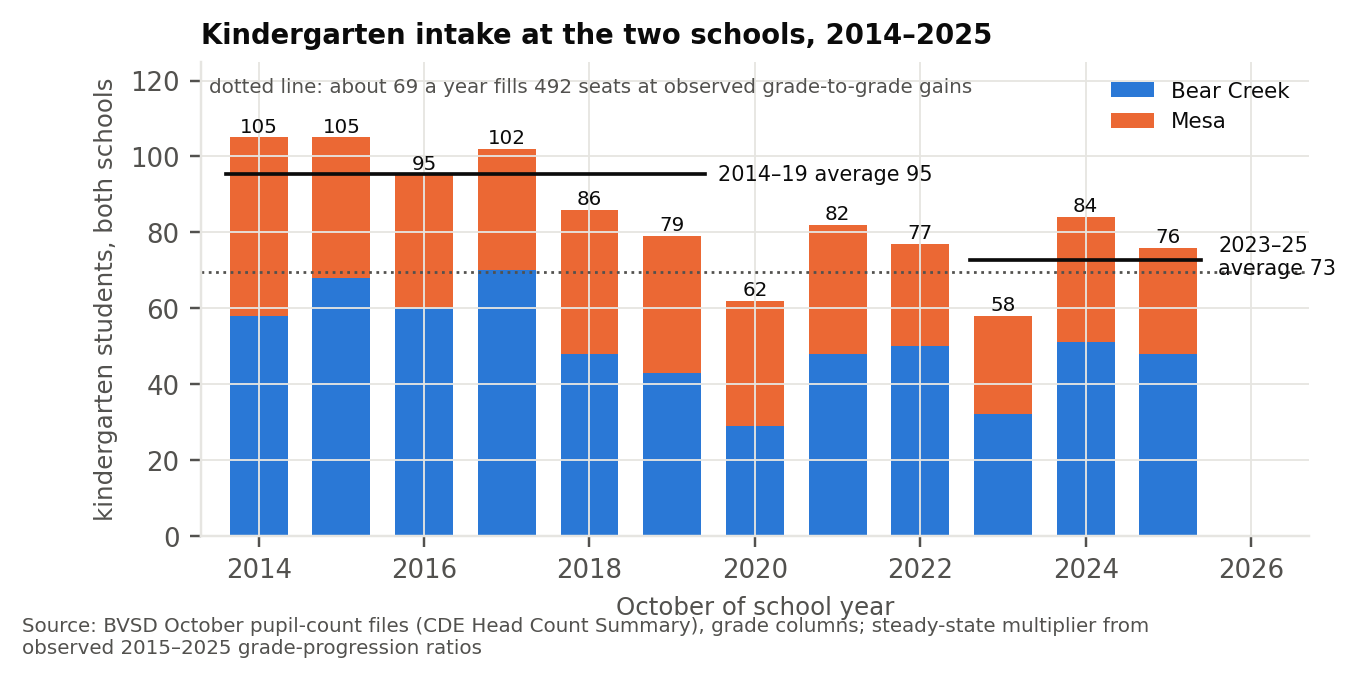
\includegraphics[width=0.9\textwidth]{fig10_kindergarten.png}
\caption{Kindergarten intake at the two schools fell from about 100 a year to about 75, then flattened after 2020.}\label{fig:kinder}\end{figure}

\begin{table}[htbp]\centering\small
\caption{Independent projection for 2030--31 (students, K--5), 1-in-10 low, central, 1-in-10 high.}\label{tab:model}
\begin{tabular}{lrrr}
\toprule
 & Low & Central & High \\
\midrule
Bear Creek, trend & 206 & 268 & 335 \\
Bear Creek, level & 254 & 317 & 384 \\
Mesa, trend & 157 & 180 & 207 \\
Mesa, level & 183 & 205 & 232 \\
Both schools, trend & 377 & 448 & 529 \\
Both schools, level & 448 & 523 & 604 \\
Both schools, check model & 377 & 461 & 566 \\
\midrule
BVSD Jan 2026 run, both schools & & 521 & \\
Proposal's range, merged school & 403 & & 462 \\
\bottomrule
\end{tabular}
\end{table}

\begin{table}[htbp]\centering\small
\caption{Merged school by share of Mesa's students following, 2030--31, both assumptions.}\label{tab:scen}
\begin{tabular}{lrrrrrrr}
\toprule
Assumption & Following & Central & Low & High & Above 450 & Above 492 & Below 300 \\
\midrule
Trend & 80\% & 412 & 343 & 490 & 26\% & 9\% & 2\% \\
Trend & 90\% & 430 & 360 & 510 & 37\% & 16\% & 1\% \\
Trend & 100\% & 448 & 377 & 529 & 49\% & 24\% & 0\% \\
Level & 80\% & 482 & 409 & 559 & 71\% & 43\% & 0\% \\
Level & 90\% & 503 & 429 & 582 & 82\% & 57\% & 0\% \\
Level & 100\% & 523 & 448 & 604 & 89\% & 70\% & 0\% \\
\bottomrule
\end{tabular}
\end{table}

\begin{table}[htbp]\centering\small
\caption{Three mutually exclusive outcomes for the merged school, 90\% following.}\label{tab:buckets}
\begin{tabular}{llrrr}
\toprule
Assumption & Year & Below 450 & 450--492 & Above 492 \\
\midrule
Trend & 2027--28 & 25\% & 45\% & 30\% \\
Level & 2027--28 & 13\% & 35\% & 52\% \\
Trend & 2030--31 & 63\% & 21\% & 16\% \\
Level & 2030--31 & 18\% & 24\% & 57\% \\
\bottomrule
\end{tabular}
\end{table}

\begin{table}[htbp]\centering\footnotesize
\caption{Conditional on the August 28, 2026 count standing in for the October 2026 count: merged school, 90\% following; percentages are shares of simulated paths under the stated assumption. ``Above 450'' and the last column are conditional.}\label{tab:cond}
\begin{tabular}{llrrrrr}
\toprule
Assumption & Year & Baseline & Conditional (low--high) & $>$450 & $>$492 base & $>$492 cond. \\
\midrule
Trend & 2027--28 & 473 & 491 (464--527) & 92\% & 30\% & 48\% \\
Level & 2027--28 & 494 & 506 (476--542) & 92\% & 52\% & 75\% \\
Trend & 2030--31 & 430 & 450 (387--513) & 50\% & 16\% & 19\% \\
Level & 2030--31 & 503 & 522 (456--590) & 92\% & 57\% & 72\% \\
\bottomrule
\end{tabular}
\end{table}

\begin{table}[htbp]\centering\footnotesize
\caption{The births assumption beside the other two: merged school, 90\% following; percentages are shares of simulated paths under the stated specification.}\label{tab:births}
\begin{tabular}{llrrrr}
\toprule
Specification & Year & Central (low--high) & $>$450 & $>$492 & Both schools \\
\midrule
Births, ratio 2014--25 & 2027--28 & 485 (449--544) & 89\% & 42\% & 505 \\
Births, ratio 2014--25 & 2030--31 & 546 (478--649) & 98\% & 83\% & 569 \\
Births, ratio 2014--23 (excludes 2024--25) & 2030--31 & 505 (460--563) & 95\% & 64\% & 526 \\
Births, ratio 2020--25 & 2030--31 & 592 (500--711) & 99\% & 92\% & 617 \\
Births, 2020--25, $B_{2025}$ at 2022--24 mean & 2030--31 & 576 (486--692) & 98\% & 88\% & 600 \\
Trend & 2030--31 & 430 (360--510) & 37\% & 16\% & 448 \\
Level & 2030--31 & 503 (429--582) & 82\% & 57\% & 523 \\
\bottomrule
\end{tabular}
\end{table}

\paragraph{Effective capacity, class size, waiting.} At effective general-education capacities of 470 and 445 (one and two rooms removed for programs), the share of simulated paths above capacity in the first year at 90\% following is 53--75\% (trend) and 75--89\% (level) (\texttt{analysis/output/table04\_effective\_capacity.csv}). Average class size at 21 rooms in 2030--31 is 20.5 (trend) or 23.9 (level); at 18 rooms 23.9 or 27.9. Re-running the model after each of 120 simulated October 2026 counts moves the 2030--31 central estimate across roughly 100 students under either assumption (\texttt{figures/fig11}): the estimate is sensitive to one more kindergarten cohort, and the August count is the first reading of it. Independent year draws for the two schools, instead of joint, leave the central estimates unchanged and narrow the 80\% range by about 15 students; the joint draw is retained as the empirically supported choice. Of nine upside cases examined (the district's projections added, resident-capture cases, the model assumptions, steady-state kindergarten cases), five reach 492 at their central value; a steady intake of about 69 a year fills 492 at observed grade-to-grade gains, and the 2023--25 average is 73.


\section{Alternatives, transportation and open questions}\label{app:alternatives}
\paragraph{The K--2 / 3--5 alternative.} The deck lists ``Reconfigure Mesa and Bear Creek into K-2 and 3-5'' first among options studied for Boulder (p.\ 56) and gives no reason for setting it aside; in October its fiscal impact was ``uncertain'' (work session slide 45). Table~\ref{tab:k25} sets the two options side by side. The alternative is not argued here to be better: it keeps two buildings, gives every family two transitions and can split siblings, and the district's June 2026 engagement summary records that families view ``grade splits'' as ``structural deal breakers'' (June 9 update, p.\ 32). Under the level assumption it meets the grade-team objective in both buildings; under the trend assumption K--2 falls short by 2030--31. What the table shows is that the comparison the Board would need in order to choose between a reversible and an irreversible option has not been published.

\begin{table}[htbp]\centering\small
\caption{Closure versus the K--2 / 3--5 reconfiguration on the district's own criteria. Model figures: 90\% following, 2030--31 (\texttt{analysis/output/table07\_reconfiguration.csv}: K--2 building 183 (trend) or 231 (level) students, 3--5 building 247 or 271).}\label{tab:k25}
\begin{tabular}{p{3.0cm}p{5.4cm}p{5.4cm}}
\toprule
Criterion & Close Mesa, merge at Bear Creek (proposed) & K--2 at one building, 3--5 at the other (studied, p.\ 56) \\
\midrule
Classes per grade & Range 403--462 gives 2.7--3.1 rounds (p.\ 51). Model: 2.9 (trend) or 3.4 (level) at 25 per class. & Not published. Model: K--2 building 2.4 (trend) or 3.1 (level); 3--5 building 3.3 or 3.6. \\
Building utilization & 82--94\% at Bear Creek (p.\ 51); Mesa building vacated. & Not published. Model: about 430--500 students across 910 seats. \\
Recurring savings & Package \$3.5--4.0M/yr (p.\ 60); no Mesa figure. & ``Uncertain'' (slide 45); not published. \\
One-time cost & Package \$7.5--10.0M $+$ \$5.0M (p.\ 60); no Mesa figure. & Not published. \\
Travel & Mesa-area students to Bear Creek; 1.5-mile rule (p.\ 64); no address count. & Every family attends both buildings over six years; not published. \\
RISE and AIM & All at Bear Creek (bvsd.org p.\ 7); rooms not published. & Not published. \\
Reversibility & Closure and boundary merger; not reversible in practice. & Grade configuration and boundaries; reversible by Board action. \\
\bottomrule
\end{tabular}
\end{table}

\paragraph{Transportation.} The deck states the eligibility rule (1.5 miles or more from the assigned school, p.\ 64) and no address count. Bear Creek runs no general-education buses today because its attendance area lies within the walk zone. About 89\% of the Mesa attendance area's land lies more than 1.5 miles from Bear Creek (attendance-area polygons; area, not addresses: most residents live in the dense northern part near both schools). The question is real for the outer part of the area, and the deck carries no cost for it.

\paragraph{Open questions the documents do not answer.}
\begin{enumerate}
\item How many classrooms do AIM and RISE occupy at Bear Creek today and after Mesa's program moves; does 492 net them out? (deck p.\ 49; bvsd.org p.\ 7)
\item What capture rate, what outside enrollment and what new-admission level do 392--445 and 403--462 assume, and is choice management applied at Bear Creek? (deck p.\ 51; FAQ p.\ 3)
\item What is the basis of the 473 and 522 residents (p.\ 51) against the matrix's 733 $\to$ 502, and of the p.\ 44 chart?
\item Read against the standalone projections, 29--59\% of Mesa's projected enrollment does not appear at Bear Creek; where do those students go, and what funding and cost follow them?
\item School-age care ``will be offered at Bear Creek'' (bvsd.org p.\ 7): with what capacity relative to two schools' demand? (FAQ p.\ 5)
\item Preschool ``will continue to be offered in the area''; where? Locations ``will be shared by Oct.\ 1'' (deck p.\ 64; FAQ p.\ 4).
\item What did the K--2 / 3--5 comparison show? (deck p.\ 56; slide 45)
\item How many Mesa-area addresses fall outside 1.5 miles of Bear Creek, and at what cost?
\item What is the Phase 4 bond project at Mesa, and does it proceed? (Bond oversight update, Feb.\ 2026)
\item Where is the September ``final plan for study'' package the June 9 update promised?
\end{enumerate}
The Boulder Reporting Lab (Aug.\ 20, 2026) reported a teacher's account of the superintendent naming a charter operator's use of a vacated building as a concern; ``decisions about the future use of buildings are not part of the Resilient Schools proposal'' (FAQ p.\ 3). Unquantified.

\paragraph{Reproducibility.}\label{app:repro}
\sloppy All scripts run from the repository root: the downloaders and parsers in \texttt{scripts/} (bvsd.org files, public documents, the matrices, the School Profile books, the weekly counts, the projection-vs-count tables, the births tables, and the earlier pupil-count, CDE and OCR parsers) and the numbered analysis scripts \texttt{analysis/01} through \texttt{analysis/20}. Figures are written to \texttt{figures/}, tables to \texttt{analysis/output/}, clean data to \texttt{data/clean/}. Random seeds are fixed. The source of this document is \texttt{report/report.tex}; \texttt{report/build.sh} renders it. Every number in the executive summary is listed with its source file in \texttt{STATUS.md}.
\end{document}
